% ============================================================================
% CSCE 763: Digital Image Processing - Homework 1
% ============================================================================

\documentclass[12pt]{article}

% ============================================================================
% PACKAGE IMPORTS
% ============================================================================
\usepackage{amsmath}
\usepackage{graphicx}
\usepackage{tikz}
\usepackage[margin=1in]{geometry}
\usepackage{xcolor}
\usepackage{enumitem}
\usepackage{tcolorbox}
\usepackage{fancyhdr}
\usepackage{booktabs}
\usepackage{array}
\usepackage{colortbl}
\usepackage{float}

% ============================================================================
% HEADER AND FOOTER SETUP
% ============================================================================
\pagestyle{fancy}
\setlength{\headheight}{14.5pt}
\fancyhf{}

\fancyhead[L]{Page \thepage}
\fancyhead[C]{CSCE 763}
\fancyhead[R]{Dr. Yan Tong}

\renewcommand{\headrulewidth}{0pt}

% ============================================================================
% TIKZ LIBRARIES
% ============================================================================
\usetikzlibrary{shapes.geometric, arrows.meta, positioning, patterns}

% --- USC Brand Colors ---
\definecolor{USC_Garnet}{HTML}{73000A}
\definecolor{USC_Black90}{HTML}{363636}
\definecolor{USC_Black10}{HTML}{ECECEC}
\definecolor{USC_Horseshoe}{HTML}{65780B}
\definecolor{USC_Atlantic}{HTML}{466A9F}

% Graphics path
\graphicspath{{figures/}}

% ============================================================================
% CUSTOM QUESTION COMMANDS
% ============================================================================
\newcommand{\question}[1]{%
  \clearpage
  \vspace{0.5cm}
  {\noindent\normalsize \textbf{#1}}
  \vspace{0.2cm}
  \hrule
  \vspace{0.1cm}
  \hrule
  \vspace{0.3cm}
}

% ============================================================================
% DOCUMENT INFORMATION
% ============================================================================

\title{CSCE 763: Digital Image Processing \\ Homework \#1}
\author{Instructor: Dr. Yan Tong \\ University of South Carolina}
\date{Due: 1:15 pm EST, Tuesday, Feb 3}

% ============================================================================
% BEGIN DOCUMENT
% ============================================================================

\begin{document}

\maketitle
\setlength{\parindent}{0pt}

\setlist[enumerate,1]{label=\arabic*.}
\setlist[enumerate,2]{label=(\alph*)}

% ============================================================================
% TABLE OF CONTENTS
% ============================================================================

\begin{center}
\begin{tcolorbox}[colback=white, colframe=gray!50!black, colbacktitle=gray!20!white,
                  coltitle=black, sharp corners, boxrule=1pt,
                  title=\Large\bfseries Table of Contents]
\begin{tabular}{p{0.82\textwidth}r}
\textbf{Problem 1: Smallest Discernible Dot (25 pts)} \dotfill & \textbf{\pageref{quest:1}} \\[0.3em]
\textbf{Problem 2: Adjacency of Image Subsets (25 pts)} & \\
\quad Part (a): 4-adjacency \dotfill & \textbf{\pageref{quest:2}} \\
\quad Part (b): 8-adjacency \dotfill & \textbf{\pageref{quest:2}} \\
\quad Part (c): m-adjacency \dotfill & \textbf{\pageref{quest:2}} \\[0.3em]
\textbf{Problem 3: Shortest Paths (25 pts)} & \\
\quad Part (a): $V = \{0, 1\}$ \dotfill & \textbf{\pageref{quest:3}} \\
\quad Part (b): $V = \{1, 2\}$ \dotfill & \textbf{\pageref{quest:3}} \\[0.3em]
\textbf{Problem 4: Set Expressions (25 pts)} \dotfill & \textbf{\pageref{quest:4}} \\
\end{tabular}
\vspace{0.2cm}
\end{tcolorbox}
\end{center}

\vspace{0.5cm}

% ============================================================================
% PROBLEM 1: Smallest Discernible Dot
% ============================================================================

\question{Problem 1: Smallest Discernible Dot (25 pts)}\label{quest:1}

Thinking purely in geometric terms, estimate the diameter of the smallest printed dot that the eye can discern if the page on which the dot is printed is 0.5\,m away from the eyes.

\textbf{Assumptions:}
\begin{enumerate}
    \item The distance between the center of the lens and the retina along the visual axis is 14\,mm.
    \item The visual system ceases to detect the dot when the image of the dot on the fovea becomes smaller than the diameter of one receptor (cone) in that area of the retina.
    \item The fovea can be modeled as a square array of dimensions $1.5\,\text{mm} \times 1.5\,\text{mm}$, and the cones (about 337{,}000 in total) and spaces between the cones are distributed uniformly throughout this array.
\end{enumerate}


% ============================================================================
% PROBLEM 2: Adjacency
% ============================================================================

\question{Problem 2: Adjacency of Image Subsets (25 pts)}\label{quest:2}

Consider the two image subsets $S_1$ and $S_2$ shown below. For $V = \{1\}$, determine whether these two subsets are (a) 4-adjacent, (b) 8-adjacent, or (c) m-adjacent.

\begin{center}
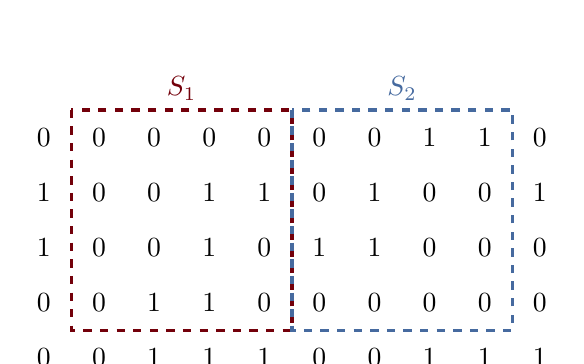
\begin{tikzpicture}[scale=0.7]
    % Row 0
    \node at (0,0) {0}; \node at (1,0) {0}; \node at (2,0) {0}; \node at (3,0) {0}; \node at (4,0) {0};
    \node at (5,0) {0}; \node at (6,0) {0}; \node at (7,0) {1}; \node at (8,0) {1}; \node at (9,0) {0};
    % Row 1
    \node at (0,-1) {1}; \node at (1,-1) {0}; \node at (2,-1) {0}; \node at (3,-1) {1}; \node at (4,-1) {1};
    \node at (5,-1) {0}; \node at (6,-1) {1}; \node at (7,-1) {0}; \node at (8,-1) {0}; \node at (9,-1) {1};
    % Row 2
    \node at (0,-2) {1}; \node at (1,-2) {0}; \node at (2,-2) {0}; \node at (3,-2) {1}; \node at (4,-2) {0};
    \node at (5,-2) {1}; \node at (6,-2) {1}; \node at (7,-2) {0}; \node at (8,-2) {0}; \node at (9,-2) {0};
    % Row 3
    \node at (0,-3) {0}; \node at (1,-3) {0}; \node at (2,-3) {1}; \node at (3,-3) {1}; \node at (4,-3) {0};
    \node at (5,-3) {0}; \node at (6,-3) {0}; \node at (7,-3) {0}; \node at (8,-3) {0}; \node at (9,-3) {0};
    % Row 4 (outside subsets)
    \node at (0,-4) {0}; \node at (1,-4) {0}; \node at (2,-4) {1}; \node at (3,-4) {1}; \node at (4,-4) {1};
    \node at (5,-4) {0}; \node at (6,-4) {0}; \node at (7,-4) {1}; \node at (8,-4) {1}; \node at (9,-4) {1};

    % S1 boundary (cols 1-4, rows 0-3)
    \draw[dashed, very thick, USC_Garnet] (0.5, 0.5) rectangle (4.5, -3.5);
    \node[above, USC_Garnet, font=\bfseries] at (2.5, 0.5) {$S_1$};

    % S2 boundary (cols 5-8, rows 0-3)
    \draw[dashed, very thick, USC_Atlantic] (4.5, 0.5) rectangle (8.5, -3.5);
    \node[above, USC_Atlantic, font=\bfseries] at (6.5, 0.5) {$S_2$};
\end{tikzpicture}
\end{center}



% ============================================================================
% PROBLEM 3: Shortest Paths
% ============================================================================

\question{Problem 3: Shortest Paths (25 pts)}\label{quest:3}

Consider the image segment shown below.

\begin{enumerate}[label=(\alph*)]
    \item Let $V = \{0, 1\}$ and compute the lengths of the shortest 4-, 8-, and m-path between $p$ and $q$. If a particular path does not exist between these two points, explain why.
    \item Repeat for $V = \{1, 2\}$.
\end{enumerate}

\begin{center}
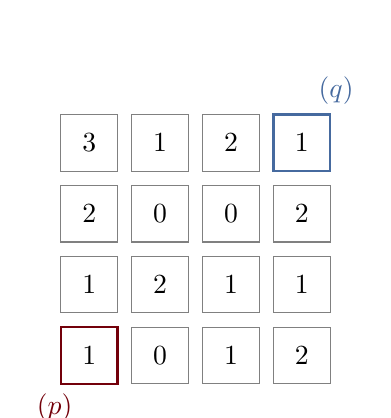
\begin{tikzpicture}[scale=0.9]
    % Row 0
    \draw[thin, gray] (-0.4,-0.4) rectangle (0.4,0.4); \node at (0,0) {3};
    \draw[thin, gray] (0.6,-0.4) rectangle (1.4,0.4); \node at (1,0) {1};
    \draw[thin, gray] (1.6,-0.4) rectangle (2.4,0.4); \node at (2,0) {2};
    \draw[thin, gray] (2.6,-0.4) rectangle (3.4,0.4); \node at (3,0) {1};
    % Row 1
    \draw[thin, gray] (-0.4,-1.4) rectangle (0.4,-0.6); \node at (0,-1) {2};
    \draw[thin, gray] (0.6,-1.4) rectangle (1.4,-0.6); \node at (1,-1) {0};
    \draw[thin, gray] (1.6,-1.4) rectangle (2.4,-0.6); \node at (2,-1) {0};
    \draw[thin, gray] (2.6,-1.4) rectangle (3.4,-0.6); \node at (3,-1) {2};
    % Row 2
    \draw[thin, gray] (-0.4,-2.4) rectangle (0.4,-1.6); \node at (0,-2) {1};
    \draw[thin, gray] (0.6,-2.4) rectangle (1.4,-1.6); \node at (1,-2) {2};
    \draw[thin, gray] (1.6,-2.4) rectangle (2.4,-1.6); \node at (2,-2) {1};
    \draw[thin, gray] (2.6,-2.4) rectangle (3.4,-1.6); \node at (3,-2) {1};
    % Row 3
    \draw[thin, gray] (-0.4,-3.4) rectangle (0.4,-2.6); \node at (0,-3) {1};
    \draw[thin, gray] (0.6,-3.4) rectangle (1.4,-2.6); \node at (1,-3) {0};
    \draw[thin, gray] (1.6,-3.4) rectangle (2.4,-2.6); \node at (2,-3) {1};
    \draw[thin, gray] (2.6,-3.4) rectangle (3.4,-2.6); \node at (3,-3) {2};

    % Mark p and q
    \node[below left, USC_Garnet, font=\bfseries] at (-0.1, -3.4) {$(p)$};
    \node[above right, USC_Atlantic, font=\bfseries] at (3.1, 0.4) {$(q)$};

    % Highlight p and q
    \draw[thick, USC_Garnet] (-0.4, -3.4) rectangle (0.4, -2.6);
    \draw[thick, USC_Atlantic] (2.6, -0.4) rectangle (3.4, 0.4);
\end{tikzpicture}
\end{center}


% ============================================================================
% PROBLEM 4: Set Expressions
% ============================================================================

\question{Problem 4: Set Expressions (25 pts)}\label{quest:4}

Give expressions for the sets shown shaded in the following figure in terms of sets $A$, $B$, and $C$. The shaded areas in each figure constitute one set, so give one expression for each of the three figures.

% --- Individual shapes A, B, C ---
\begin{center}
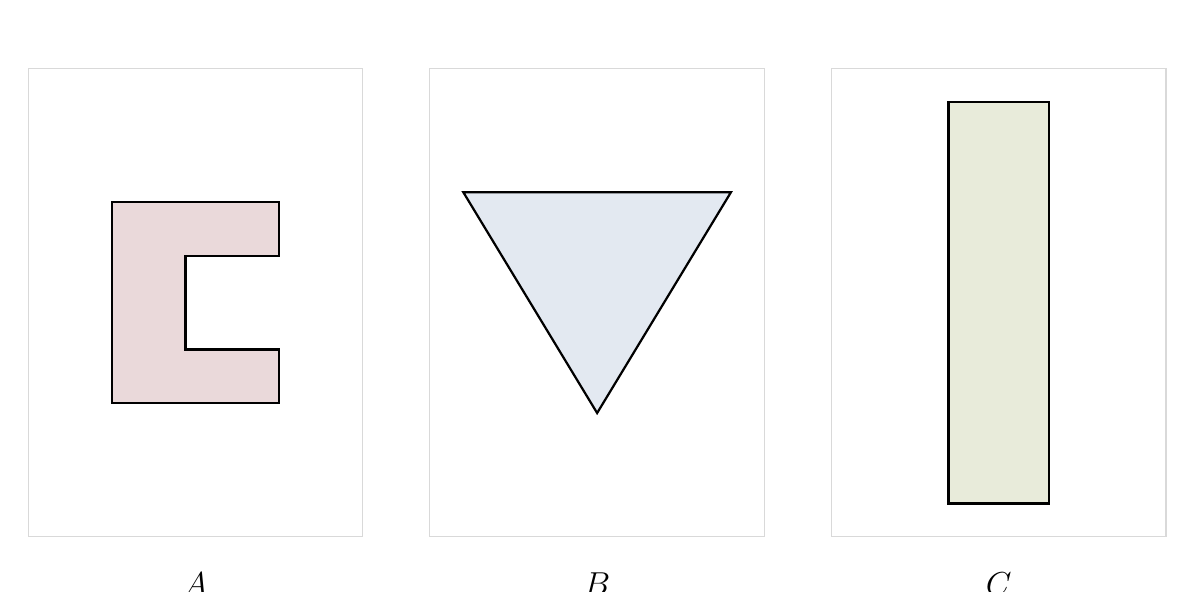
\begin{tikzpicture}[scale=0.85]

    % All columns are 5 units wide, centered at x = 2.5, 8.5, 14.5

    % === Shape A (width 2.5, height 3) -> center at (2.5, 3) ===
    \begin{scope}[shift={(0,0)}]
        \draw[gray!30, thin] (0,-0.5) rectangle (5,6.5);
        \fill[USC_Garnet!15] (1.25,1.5) -- (3.75,1.5) -- (3.75,2.3) -- (2.35,2.3) -- (2.35,3.7) -- (3.75,3.7) -- (3.75,4.5) -- (1.25,4.5) -- cycle;
        \draw[thick] (1.25,1.5) -- (3.75,1.5) -- (3.75,2.3) -- (2.35,2.3) -- (2.35,3.7) -- (3.75,3.7) -- (3.75,4.5) -- (1.25,4.5) -- cycle;
        \node[font=\large\bfseries] at (2.5, -1.2) {$A$};
    \end{scope}

    % === Shape B (width 4, height 3.3) -> center at (8.5, 3) ===
    \begin{scope}[shift={(6,0)}]
        \draw[gray!30, thin] (0,-0.5) rectangle (5,6.5);
        \fill[USC_Atlantic!15] (0.5,4.65) -- (4.5,4.65) -- (2.5,1.35) -- cycle;
        \draw[thick] (0.5,4.65) -- (4.5,4.65) -- (2.5,1.35) -- cycle;
        \node[font=\large\bfseries] at (2.5, -1.2) {$B$};
    \end{scope}

    % === Shape C (width 1.5, height 6) -> center at (14.5, 3) ===
    \begin{scope}[shift={(12,0)}]
        \draw[gray!30, thin] (0,-0.5) rectangle (5,6.5);
        \fill[USC_Horseshoe!15] (1.75,0) -- (3.25,0) -- (3.25,6) -- (1.75,6) -- cycle;
        \draw[thick] (1.75,0) -- (3.25,0) -- (3.25,6) -- (1.75,6) -- cycle;
        \node[font=\large\bfseries] at (2.5, -1.2) {$C$};
    \end{scope}

\end{tikzpicture}
\end{center}

% Pre-computed world coordinates:
% A: (0,3) -- (2.5,3) -- (2.5,3.8) -- (1.1,3.8) -- (1.1,5.2) -- (2.5,5.2) -- (2.5,6) -- (0,6) -- cycle
% B: (-0.99,3.96) -- (3.41,3.96) -- (1.21,0.33) -- cycle
% C: (2,0.2) -- (3.5,0.2) -- (3.5,6.2) -- (2,6.2) -- cycle

% Macros for shape paths
\newcommand{\pathA}{(0,3) -- (2.5,3) -- (2.5,3.8) -- (1.1,3.8) -- (1.1,5.2) -- (2.5,5.2) -- (2.5,6) -- (0,6) -- cycle}
\newcommand{\pathB}{(-0.99,3.96) -- (3.41,3.96) -- (1.21,0.33) -- cycle}
\newcommand{\pathC}{(2,0.2) -- (3.5,0.2) -- (3.5,6.2) -- (2,6.2) -- cycle}

\vspace{0.5cm}
\hrule
\vspace{0.5cm}

% --- Three shaded figures ---
\begin{center}
\begin{tikzpicture}[scale=0.8]

    % ============================
    % FIGURE (i): A ∩ B ∩ C
    % ============================
    \begin{scope}[shift={(0,0)}]
        \begin{scope}
            \clip \pathA;
            \clip \pathB;
            \clip \pathC;
            \fill[gray!40] (-2,-1) rectangle (5,7);
        \end{scope}
        \draw[thick] \pathA;
        \draw[thick] \pathB;
        \draw[thick] \pathC;
        \node[below] at (1.5, -0.5) {(i)};
    \end{scope}

    % ============================
    % FIGURE (ii): (A∩B) ∪ (B∩C) ∪ (A∩C)
    % ============================
    \begin{scope}[shift={(8,0)}]
        % Shade A ∩ B
        \begin{scope}
            \clip \pathA;
            \clip \pathB;
            \fill[gray!40] (-2,-1) rectangle (5,7);
        \end{scope}
        % Shade B ∩ C
        \begin{scope}
            \clip \pathB;
            \clip \pathC;
            \fill[gray!40] (-2,-1) rectangle (5,7);
        \end{scope}
        % Shade A ∩ C
        \begin{scope}
            \clip \pathA;
            \clip \pathC;
            \fill[gray!40] (-2,-1) rectangle (5,7);
        \end{scope}
        \draw[thick] \pathA;
        \draw[thick] \pathB;
        \draw[thick] \pathC;
        \node[below] at (1.5, -0.5) {(ii)};
    \end{scope}

    % ============================
    % FIGURE (iii): (B ∩ A^c ∩ C^c) ∪ (A ∩ C ∩ B^c)
    % ============================
    \begin{scope}[shift={(16,0)}]
        % Shade B
        \begin{scope}
            \clip \pathB;
            \fill[gray!40] (-2,-1) rectangle (5,7);
        \end{scope}
        % Remove B ∩ A
        \begin{scope}
            \clip \pathB;
            \clip \pathA;
            \fill[white] (-2,-1) rectangle (5,7);
        \end{scope}
        % Remove B ∩ C
        \begin{scope}
            \clip \pathB;
            \clip \pathC;
            \fill[white] (-2,-1) rectangle (5,7);
        \end{scope}
        % Shade A ∩ C
        \begin{scope}
            \clip \pathA;
            \clip \pathC;
            \fill[gray!40] (-2,-1) rectangle (5,7);
        \end{scope}
        % Remove A ∩ C ∩ B
        \begin{scope}
            \clip \pathA;
            \clip \pathC;
            \clip \pathB;
            \fill[white] (-2,-1) rectangle (5,7);
        \end{scope}
        \draw[thick] \pathA;
        \draw[thick] \pathB;
        \draw[thick] \pathC;
        \node[below] at (1.5, -0.5) {(iii)};
    \end{scope}

\end{tikzpicture}
\end{center}


% ============================================================================
% END OF DOCUMENT
% ============================================================================

\end{document}
